\lstset{language=VBScript,
        basicstyle=\footnotesize\ttfamily,
        breaklines=true,
        tabsize=2,
        numbers=left,
        numberstyle=\tiny,
        numbersep=7pt,
        showspaces=false,
        keywordstyle=\color{Blue}\textbf,
        commentstyle=\color{Red}\emph,
        showstringspaces=false,
        stringstyle=\color{BurntOrange}
        }
\section{Instrukcja użytkownika}
%\subsection{Specyfikacja zewnętrzna}
Zaimplementowana przez autora wizualizacja ma na~celu zobrazowanie działania modelu oraz umożliwienie operatorowi wpływania na~jego działanie. Kolejne podrozdziały zawierają opis specyfikacji zewnętrznej oraz wewnętrznej. Część odnosząca się do specyfikacji zewnętrznej jest skróconą instrukcją obsługi użytkownika. Specyfikacja wewnętrzna jest opisem, jak zostały zrealizowane poszczególne elementy~i~w jaki sposób wizualizacja współpracuje ze~sterownikiem.


Specyfikacja zewnętrzna przedstawiona w dalszej części podrozdziału stanowi skróconą instrukcję obsługi wizualizacji oraz opis możliwości oferowanych przez poszczególne ekrany.

Autor projektu wykorzystał w~swojej pracy szereg elementów dostępnych standardowo w~środowisku Simatic WinCC flexible. Podstawowymi elementami sterującymi są przyciski w~trybie tekstowym oraz przeźroczystym. Głównymi obiektami służącymi do prezentacji informacji są: pola tekstowe, pola wejściowo-wyjściowe oraz pola daty i~godziny. Dodatkowo celem uatrakcyjnienia wizualizacji wykorzystane zostały suwaki (ang. \emph{slider}), obrazki oraz zegarek. 

Obsługa tej części projektu jest realizowana za pomocą myszy i~klawiatury podłączonych do~komputera. Za~pomocą klawiatury wybieramy interesujący nas ekran lub wprowadzamy żądaną wartość pozycji docelowej na~ekranie testowania trybu automatycznego.

Wszystkie ekrany wizualizacji są tworzone na podstawie szablonu. Wszystkie przyciski widoczne w~górnej części Rysunku~\ref{template} są powiązane z~wybranymi klawiszami na klawiaturze z~zakresu F1~do~F12. 
Użycie pierwszych 6 przycisków lub związanych z~nimi klawiszy F1~-~F6 powoduje zmianę aktualnie wyświetlanego ekranu.
Przycisk „Koniec" \space na wizualizacji oraz powiązany z~nim klawisz F7 po~aktywowaniu powodują zamknięcie wizualizacji poprzez wywołanie funkcji standardowej StopRuntime.

Dodatkowo do~przycisków F9~-~F12 została przypisana zmiana stanu zmiennej \emph{EmergencyStop}, która pozwala na~awaryjne zatrzymanie pracy robota w~dowolnym momencie. Modyfikowanie wartości zmiennej odpowiadającej za~awaryjne zatrzymanie pracy może się również odbywać poprzez kliknięcie na~kontrolkę znajdującą się w~prawym dolnym rogu każdego ekranu.
Ekrany dostępne w wizualizacji oraz klawisze funkcyjne z nimi związane:
\begin{itemize} 
\item Ekran powitalny - F1,
\item Stan robota - F2,
\item Stan magazynu i testowanie obsługi - F3,
\item Testowanie sterowania ręcznego z pilota podłączonego do sterownika - F4,
\item Testowanie sterowania ręcznego z poziomu wizualizacji - F5,
\item Testowanie sterowania automatycznego - F6.
\end{itemize}
\indent
\indent Poszczególne ekrany zostaną szczegółowo opisane w kolejnych podrozdziałach.
\begin{figure}[!htb] 	\centering 	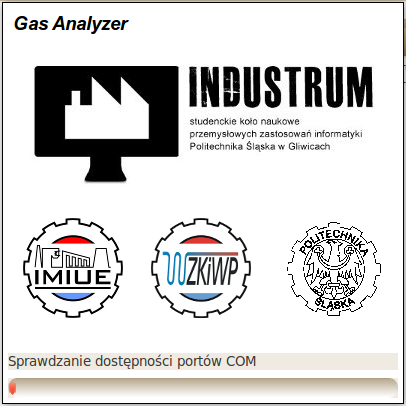
\includegraphics[width=0.5\textwidth]{images/splashScreen.png} \caption{Okno ładowania} \label{template} \end{figure}
\subsubsection{Ekran powitalny}
Bezpośrednio po~uruchomieniu wizualizacji użytkownik zobaczy ekran powitalny taki jak na Rysunku~\ref{vis1} zawierający informacje o~autorze projektu, osobie kierującej projektem (promotorze) oraz informację o~przeznaczeniu wizualizacji wraz ze~zdjęciem modelu. Dodatkowo na~ekranie tym umieszczony został zegar analogowy i~cyfrowy oraz aktualna data.
\begin{figure}[!htb]
\centering 		
  \subfloat[Windows]{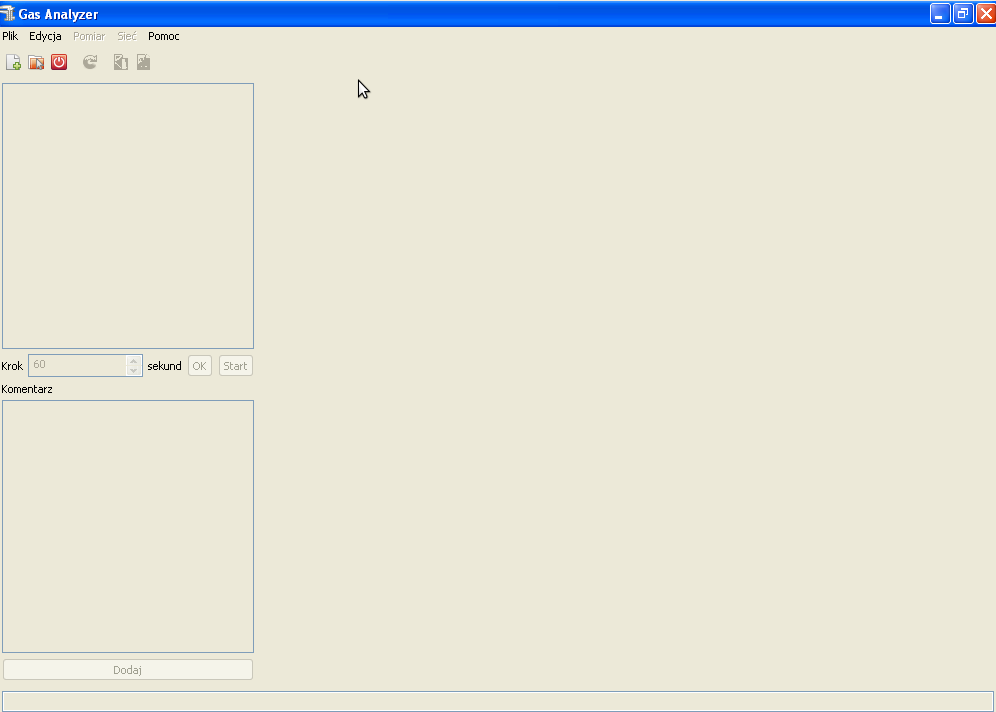
\includegraphics[width=0.45\textwidth]{images/mainW.png}}                
  \subfloat[Linux]{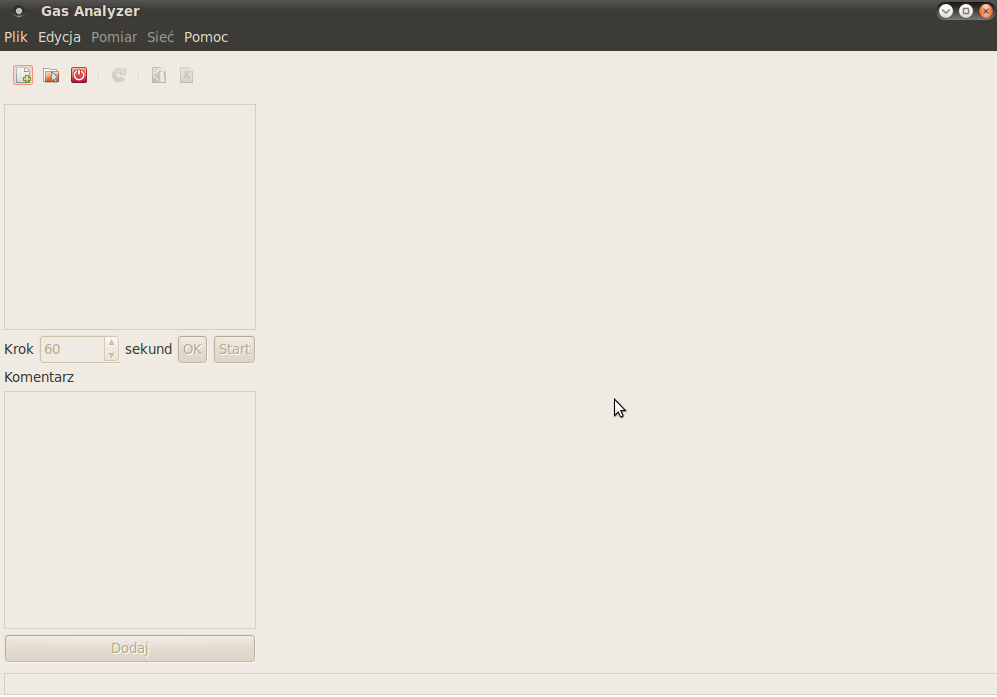
\includegraphics[width=0.45\textwidth]{images/mainL.png}}
\caption{Okno główne} 	
\label{vis1}
\end{figure}
\subsubsection{Stan robota}
Ekran przedstawiający aktualny stan robota widoczny jest na Rysunku~\ref{vis2}. Prezentuje on informacje o~stanie poszczególnych silników oraz o~trybie pracy modelu. Na~ekranie zobaczyć można informacje o tym, czy silnik nie osiągnął swojej pozycji minimalnej lub maksymalnej, czy nie występuje sygnał z~krańcówki lub z~czujnika impulsów oraz aktualne położenie każdego silnika w~formie liczbowej i~jako wypadkowa na~suwaku. Ponadto na ekranie tym znajdują się informacje o~ewentualnych błędach. Jeśli dany błąd wystąpi w~sterowniku to na ekranie pojawi się pole tekstowe z~jego treścią. Klikając na~pole z~treścią błędu wymuszona jest zmiana flagi odpowiedzialnej za~wystąpienie, co~skutkuje zniknięciem błędu z~ekranu. W~sytuacji gdy błąd nie znika oznacza to, że~występuje on~nadal w~sterowniku.
\begin{figure}[!htb]	
\centering 	
  \subfloat[Bez połączenia ze sterownikiem]{\includegraphics[width=0.45\textwidth]{images/vis2off.png}}                
  \subfloat[Z podłączonym sterownikiem]{\includegraphics[width=0.45\textwidth]{images/vis2on.png}}
\caption{Ekran prezentujący stan robota} 
\label{vis2}
\end{figure}
\subsubsection{Stan magazynu i testowanie obsługi}
Najważniejszym ekranem w~całej wizualizacji jest ekran zawierający stan magazynu, pozostałe pełnią bowiem role informacyjne lub testowe. Ekran ten składa się z~kilku bardzo ważnych części, które można zaobserwować na Rysunku~\ref{vis3}. 

W~lewej górnej części widać kolejkę zadań do wykonania wraz z~jej aktualną długością. Długość podana jest w nawiasie przy nagłówku „Kolejka". Poniżej tego nagłówka widocznych jest 11~początkowych elementów kolejki. Każdy element kolejki składa się z~indeksu pozycji w~magazynie oraz wartości bool decydującej, czy element będzie zabrany czy położony. Pod prezentowaną kolejką widnieje przycisk „\noindent Start", który powoduje rozpoczęcie wykonywania zadań dodanych wcześniej przez użytkownika do~kolejki. 

Na środku znajdują się 24~prostokąty obrazujące szufladki w~magazynie. Kolor pola informuje o~tym, czy jest ono zajęte czy wolne. Kolor zielony oznacza, że dana szufladka jest pusta, natomiast prostokąt w~kolorze czerwonym oznacza, że dana szufladka jest już zajęta. Na~każdym polu znajdują się przycisk „Weź"~oraz~„Połóż". Podobne do pól magazynu są pola wejściowe oraz wyjściowe. Przy polach tych dodatkowo znajdują się przyciski, które umożliwiają zasymulowanie położenia produktu na~platformie wejściowej oraz odbiór produktu z~platformy wyjściowej. Po prawej stronie u~góry widać grupę przycisków służących do wybierania indeksu elementu w~specyficzny sposób. Elementy wyżej służą do~wybierania elementów najbliżej lub najdalej położonych w tablicy. Przyciski poniżej służą do wybierania elementu najmłodszego lub najstarszego włożonego wcześniej do~magazynu. 

Wszystkie pola magazynu oraz platformy wejściowa i~wyjściowa posiadają dodatkową informację o~dacie i~godzinie ostatniego użycia. Po umieszczeniu w danej komórce lub zabraniu z~niej produktu, sterownik zapisuje w~pamięci informację o~dacie i~godzinie tego zdarzenia. 

Dolna część ekranu pełni tylko funkcję informacyjną. Po~lewej stronie znajdują się godzina oraz data odczytane z~komputera lub panelu operatorskiego i~sterownika przemysłowego. Z~prawej natomiast znajdują się informacje o~aktualnym położeniu poszczególnych silników w~formie wartości liczbowej. 

Ostatnim elementem znajdującym się na~tym~ekranie jest informacja dla użytkownika o~ewentualnych błędach. Zasada działania tych informacji jest taka sama jak na ekranie z informacjami o~stanie robota, co~zostało opisane przez autora wcześniej.
\begin{figure}[!htb]
\centering 	
  \subfloat[Bez połączenia ze sterownikiem]{\includegraphics[width=0.45\textwidth]{images/vis3off.png}}                
  \subfloat[Z podłączonym sterownikiem]{\includegraphics[width=0.45\textwidth]{images/vis3on.png}}
\caption{Ekran prezentujący stan magazynu i umożliwiający obsługę} 
\label{vis3}
\end{figure}
\subsubsection{Testowanie sterowania ręcznego z poziomu wizualizacji}
Testowanie trybu manualnego z~poziomu wizualizacji polega na~wybieraniu kierunku pracy oraz załączaniu poszczególnych silników wykorzystując do tego celu 8~przycisków znajdujących się na ekranie (4~grupy po 2~przyciski na każdy silnik). Na~ekranie oprócz wymienionych już przycisków znajdują się również informacje o~tym, jaki jest stan poszczególnych silników, jakie jest ich bieżące położenie, czy któryś z~nich nie osiągnął swojego minimum lub maksimum oraz sygnały z~zamontowanych na robocie czujników. Ekran ten został zaprezentowany na Rysunku~\ref{vis4}.
Dodatkowo do ekranu tego zostały przypisane klawisze ułatwiające obsługę. Na Rysunku~\ref{template} pokazane zostały przyciski związane ze~wszystkimi ekranami, natomiast przyciski przypisane tylko do wybranego ekranu mają żółty kolor trójkąta informacyjnego, co zauważyć można na Rysunku~\ref{manvis}. Dla odróżnienia klawiszy globalnych od tych dla konkretnego ekranu autor postanowił wykorzystać kombinacje klawiszy Shift+F1 do Shift+F8. Dla sterowania silnikiem Lift wykorzystano kombinację Shift+F1 (start) i~Shift+F2 (kierunek), dla silnika Arm Shift+F3 (start) i~Shift+F4 (kierunek), dla silnika Rotate Shift+F5 (start) i~Shift+F6 (kierunek) oraz dla silnika Grab Shift+F7 (start) i~Shift+F8 (kierunek).
\begin{figure}[!htb] 	\centering 	\includegraphics[width=0.7\textwidth]{images/manualvis.png} 	\caption{Widok dodatkowych klawiszy przypisanych do ekranu testowania sterowania ręcznego z poziomu wizualizacji} \label{manvis} \end{figure}
\begin{figure}[!htb]
\centering 	
  \subfloat[Bez połączenia ze sterownikiem]{\includegraphics[width=0.45\textwidth]{images/vis4off.png}}                
  \subfloat[Z podłączonym sterownikiem]{\includegraphics[width=0.45\textwidth]{images/vis4on.png}}
\caption{Ekran umożliwiający testowanie sterowania ręcznego z poziomu wizualizacji} 
\label{vis4}
\end{figure}
\subsubsection{Testowanie sterowania ręcznego z pilota podłączonego do sterownika}
Podobnie jak w~przypadku testowania trybu manualnego z~poziomu wizualizacji w~trybie manualnym z~pilota sterujemy pracą robota za~pomocą przycisków. Tym razem przyciski znajdujące się na~ekranie pełnią tylko rolę informacyjną na~temat stanu tych znajdujących się na~pilocie podłączonym bezpośrednio do~sterownika. Sterowanie faktyczne odbywa się za~pomocą przycisków znajdujących się na~pilocie. Oprócz tego na~ekranie widocznym na Rysunku~\ref{vis5} znajdują się takie same informacje jak w~przypadku ekranu ze~sterowania z~poziomu wizualizacji.
\begin{figure}[!htb]
\centering 	
  \subfloat[Bez połączenia ze sterownikiem]{\includegraphics[width=0.45\textwidth]{images/vis5off.png}}                
  \subfloat[Z podłączonym sterownikiem]{\includegraphics[width=0.45\textwidth]{images/vis5on.png}}
\caption{Ekran umożliwiający testowanie sterowania ręcznego z pilota podłączonego do sterownika} 
\label{vis5}
\end{figure}
\subsubsection{Testowanie sterowania automatycznego}
Testowanie trybu automatycznego polega na~wprowadzaniu przez użytkownika wartości docelowej dla poszczególnych silników. Oprócz pól do wprowadzania tych wartości widocznych na Rysunku~\ref{vis6} użytkownik widzi takie same informacje jak dla testowania trybów sterowania ręcznego.
\begin{figure}[!htb]
\centering 	
  \subfloat[Bez połączenia ze sterownikiem]{\includegraphics[width=0.45\textwidth]{images/vis6off.png}}                
  \subfloat[Z podłączonym sterownikiem]{\includegraphics[width=0.45\textwidth]{images/vis6on.png}}
\caption{Ekran umożliwiający testowanie sterowania automatycznego} 
\label{vis6}
\end{figure}
\subsection{Specyfikacja wewnętrzna}
Wizualizacja komunikuje się z~komputera klasy~PC ze~sterownikiem za~pośrednictwem protokołu Ethernet w~sieci lokalnej.
Odniesienia do~odpowiednich adresów w~pamięci sterownika dokonywane są za~pomocą nazw symbolicznych zdefiniowanych w~tablicy Tags. Do działania wizualizacja używa tylko jednej zmiennej wewnętrznej i~jest~to zmienna tablicowa \emph{MagazynDTEnable} z elementami typu bool. Elementy te odpowiadają za~wyświetlanie dat oraz godzin na~ekranie ze~stanem magazynu po~kliknięciu na~wybraną komórkę. Obsługa wyświetlania dat polega na tym, że po kliknięciu w wybrane pole ustawiana jest odpowiednia zmienna w~tej tablicy na~wartośc \emph{true}, a~po zwolnieniu klawisza myszki na wartość \emph{false}. Za zmiany te odpowiadają niewidzialne przyciski umieszczone na~tych polach.

Wizualizacja wpływa na pracę sterownika poprzez zmianę pojedynczych bitów za~pomocą umieszczonych na~ekranie przycisków. Wpływa ona również poprzez modyfikowanie wybranych zmiennych odpowiadających pozycjom docelowym lub poprzez dodawanie odpowiednich zadań do~kolejki. Bardziej zaawansowane operacje zostały zrealizowane za~pomocą skryptów napisanych w~języku VBScript, które są bardzo prostą i~szybką opcją wykonywania bardziej zaawansowanych czynności. 
\newpage
Skrypt BDScirpt wywołuje, poprzez ustawienie odpowiednich bitów w sterowniku, funkcję wybierającą najbliższą lub najdalszą pustą lub zajętą komórkę w~magazynie. \\[1mm]
\begin{lstlisting}[caption={BDScript}]
If i=1 Then
	SmartTags("BD") = True
	SmartTags("BDEn") = True
	SmartTags("AddBoolWarehouse") = True
ElseIf i=2 Then
	SmartTags("BD") = True
	SmartTags("BDEn") = True
	SmartTags("AddBoolWarehouse") = False
ElseIf i=3 Then
	SmartTags("BD") = False
	SmartTags("BDEn") = True
	SmartTags("AddBoolWarehouse") = True
Else
	SmartTags("BD") = False
	SmartTags("BDEn") = True
	SmartTags("AddBoolWarehouse") = False
End If \end{lstlisting}

Skrypt NNScirpt wywołuje w sterowniku wybranie najstarszej lub najmłodszej zajętej komórki z~magazynu i~dodanie jej do~kolejki zadań.\\[1mm]
\begin{lstlisting}[caption={NNScript}]
If i=1 Then 
	SmartTags("NN") = True
	SmartTags("NNEn") = True
Else 
	SmartTags("NN") = False
	SmartTags("NNEn") = True
End If 
\end{lstlisting}

Po wybraniu opcji „Połóż"~lub~„Weź"~są~wywoływane odpowiednio skrypty MagazynPush lub MagazynTake. Skrypty~te~powodują dodanie odpowiedniego indeksu oraz ruchu chwytaka do kolejki zadań. \\[1mm]
\begin{lstlisting}[caption={MagazynPush}]
SmartTags("AddedIndex") = i
SmartTags("AddBoolWarehouse") = False
SmartTags("AddQueue") = True
\end{lstlisting}

\begin{lstlisting}[caption={MagazynTake}]
SmartTags("AddedIndex") = i
SmartTags("AddBoolWarehouse") = True
SmartTags("AddQueue") = True
\end{lstlisting}
